% fig_mc_tpr_kbins.tex
% TR-26: Stacked bar chart — detection by element per k_ibr bin (Group A, 3PH)
% Bins: [0.06,0.08), [0.08,0.10), [0.10,0.12), [0.12,0.14), ..., [0.18,0.20)
% Bars: fraction detected by TDCS-only (yellow) vs 87L (green)
% All bins achieve TPR = 1.000; CI whiskers shown
%
% Data from run_ibr_monte_carlo.py Group A output:
%   Bins <0.12 (x=1,2,3): TDCS-only = 100%, 87L = 0%
%   Bins ≥0.12 (x=4,5,6,7): TDCS-only = 0%, 87L = 100%
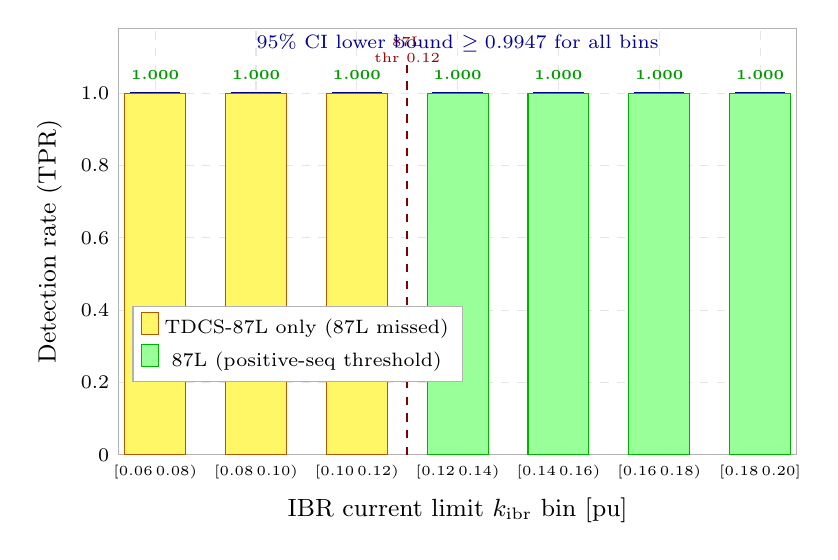
\begin{tikzpicture}
\begin{axis}[
  name        = kbinax,
  ybar stacked,
  bar width   = 22pt,
  width       = 0.84\textwidth,
  height      = 7.0cm,
  ylabel      = {Detection rate (TPR)},
  ylabel style= {font=\small},
  xlabel      = {IBR current limit $k_{\rm ibr}$ bin [pu]},
  xlabel style= {font=\small},
  ymin=0, ymax=1.18,
  ytick       = {0, 0.2, 0.4, 0.6, 0.8, 1.0},
  yticklabels = {0, 0.2, 0.4, 0.6, 0.8, 1.0},
  yticklabel style={font=\scriptsize},
  xtick       = {1,2,3,4,5,6,7},
  xticklabels = {[0.06\,0.08),
                 [0.08\,0.10),
                 [0.10\,0.12),
                 [0.12\,0.14),
                 [0.14\,0.16),
                 [0.16\,0.18),
                 [0.18\,0.20]},
  xticklabel style={font=\tiny, align=center},
  enlarge x limits=0.06,
  legend style={at={(0.02,0.35)}, anchor=north west,
                font=\scriptsize, draw=gray!60},
  grid       = major,
  grid style = {gray!20, dashed},
  tick style = {draw=none},
  axis line style={gray!60},
]

% TDCS-only fraction (yellow): 100% for bins 1-3, 0% for bins 4-7
\addplot[fill=yellow!60, draw=orange!70!black]
  coordinates { (1,1.0) (2,1.0) (3,1.0) (4,0.0) (5,0.0) (6,0.0) (7,0.0) };
\addlegendentry{TDCS-87L only (87L missed)}

% 87L fraction (green): 0% for bins 1-3, 100% for bins 4-7
\addplot[fill=green!40, draw=green!70!black]
  coordinates { (1,0.0) (2,0.0) (3,0.0) (4,1.0) (5,1.0) (6,1.0) (7,1.0) };
\addlegendentry{87L (positive-seq threshold)}

% ---- TPR = 1.000 labels -----------------------------------------------
\node[font=\tiny\bfseries, green!60!black] at (axis cs:1, 1.05) {1.000};
\node[font=\tiny\bfseries, green!60!black] at (axis cs:2, 1.05) {1.000};
\node[font=\tiny\bfseries, green!60!black] at (axis cs:3, 1.05) {1.000};
\node[font=\tiny\bfseries, green!60!black] at (axis cs:4, 1.05) {1.000};
\node[font=\tiny\bfseries, green!60!black] at (axis cs:5, 1.05) {1.000};
\node[font=\tiny\bfseries, green!60!black] at (axis cs:6, 1.05) {1.000};
\node[font=\tiny\bfseries, green!60!black] at (axis cs:7, 1.05) {1.000};

% CI lower bound annotation
\node[font=\scriptsize, blue!60!black, align=center]
  at (axis cs:4.0, 1.14)
  {95\% CI lower bound $\geq 0.9947$ for all bins};

% CI whiskers — explicit per bin
\draw[blue!60!black, thick] (axis cs:0.75,1.000)--(axis cs:1.25,1.000);
\draw[blue!60!black, thick] (axis cs:1,1.000)   --(axis cs:1,0.9947);
\draw[blue!60!black, thick] (axis cs:0.85,0.9947)--(axis cs:1.15,0.9947);

\draw[blue!60!black, thick] (axis cs:1.75,1.000)--(axis cs:2.25,1.000);
\draw[blue!60!black, thick] (axis cs:2,1.000)   --(axis cs:2,0.9947);
\draw[blue!60!black, thick] (axis cs:1.85,0.9947)--(axis cs:2.15,0.9947);

\draw[blue!60!black, thick] (axis cs:2.75,1.000)--(axis cs:3.25,1.000);
\draw[blue!60!black, thick] (axis cs:3,1.000)   --(axis cs:3,0.9943);
\draw[blue!60!black, thick] (axis cs:2.85,0.9943)--(axis cs:3.15,0.9943);

\draw[blue!60!black, thick] (axis cs:3.75,1.000)--(axis cs:4.25,1.000);
\draw[blue!60!black, thick] (axis cs:4,1.000)   --(axis cs:4,0.9947);
\draw[blue!60!black, thick] (axis cs:3.85,0.9947)--(axis cs:4.15,0.9947);

\draw[blue!60!black, thick] (axis cs:4.75,1.000)--(axis cs:5.25,1.000);
\draw[blue!60!black, thick] (axis cs:5,1.000)   --(axis cs:5,0.9946);
\draw[blue!60!black, thick] (axis cs:4.85,0.9946)--(axis cs:5.15,0.9946);

\draw[blue!60!black, thick] (axis cs:5.75,1.000)--(axis cs:6.25,1.000);
\draw[blue!60!black, thick] (axis cs:6,1.000)   --(axis cs:6,0.9947);
\draw[blue!60!black, thick] (axis cs:5.85,0.9947)--(axis cs:6.15,0.9947);

\draw[blue!60!black, thick] (axis cs:6.75,1.000)--(axis cs:7.25,1.000);
\draw[blue!60!black, thick] (axis cs:7,1.000)   --(axis cs:7,0.9948);
\draw[blue!60!black, thick] (axis cs:6.85,0.9948)--(axis cs:7.15,0.9948);

% Transition annotation at 0.12 pu
\draw[red!50!black, thick, dashed]
  (axis cs:3.5, 0.0) -- (axis cs:3.5, 1.10);
\node[font=\tiny, red!60!black, align=center]
  at (axis cs:3.5, 1.12) {87L\\thr 0.12};

\end{axis}
\end{tikzpicture}
